%!TEX root = ../Thesis.tex

\chapter{Effects of model and algorithm augmentations (Adam optimizer)}\label{app: Effects of common model and algorithm augmentations (Adam optimizer)}
This appendix presents the effects of common model and algorithm augmentations as in \autoref{sec: Experimental work: Effects of common model and algorithm augmentations} only here the popular Adam optimizer \cite{Kingma2014} is used instead of regular \gls{SGD}. 

For all figures, \textbf{(a)} shows the training and validation set classification accuracy of the unperturbed model while \textbf{(b)} shows the training and validation \gls{NLL} loss.

Some trends from the experiments using the \gls{SGD} optimizer are also visible when using the Adam optimizer, e.g. the effect of using batch normalization in \autoref{fig: Theory: E017-bn-analysis} and the
superiority of using antithetic sampling \autoref{fig: Theory: E019-AS-analysis}. Generally speaking however, the Adam optimizer results in more unstable learning with much larger variance within several runs using the same hyperparameters and lower final performance across the line. 

The poorer performance of Adam cannot be ruled out to be an issue related to hyperparameter choices since these were found heuristically. It did however prove significantly easier to achieve stable learning using \gls{SGD} compared to Adam. It is hypothesized that this may have to do with the variance of the stochastically estimated gradient being too high for good estimation of higher order moments, such as those used in Adam. This is in line with the discussion on the variance of the stochastic Hessian estimate presented in \autoref{sec: Theory: Taylor: Second order derivative}. It is also supported by the results in \autoref{fig: Theory: E019-AS-analysis} since the between run variance decreases when antithetic sampling is used.

\begin{figure}[bp!]
    \begin{subfigure}[b]{0.49\textwidth}
        \centering
        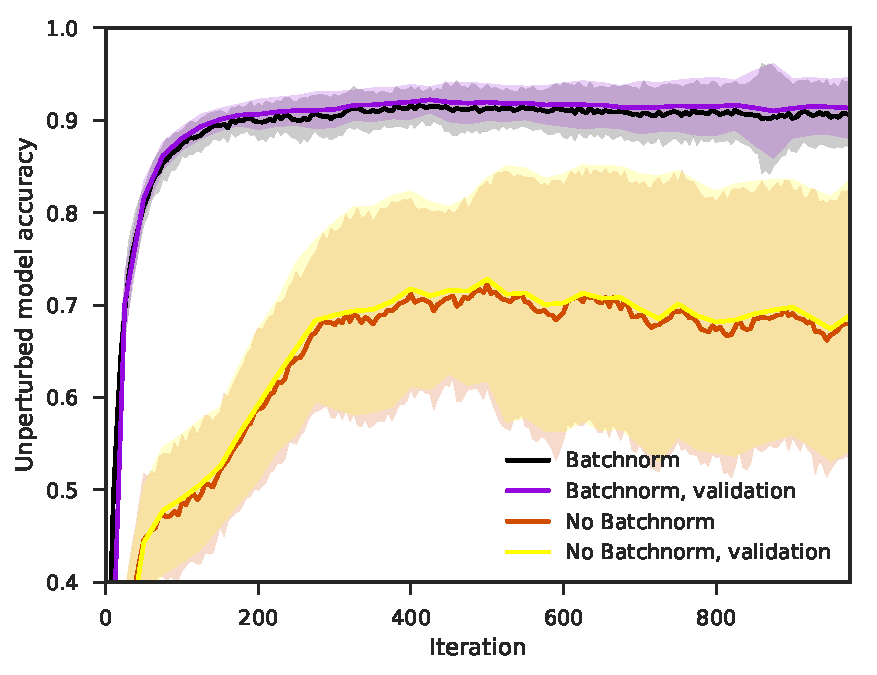
\includegraphics[height=5.8cm]{graphics/E017-bn-analysis/accuracy_unp-all-series-mean-sd.pdf}
        \caption{}
        \label{fig: Theory: E017-bn-analysis/accuracy_unp-all-series-mean-sd}
    \end{subfigure}
    \hfill
    \begin{subfigure}[b]{0.49\textwidth}
        \centering
        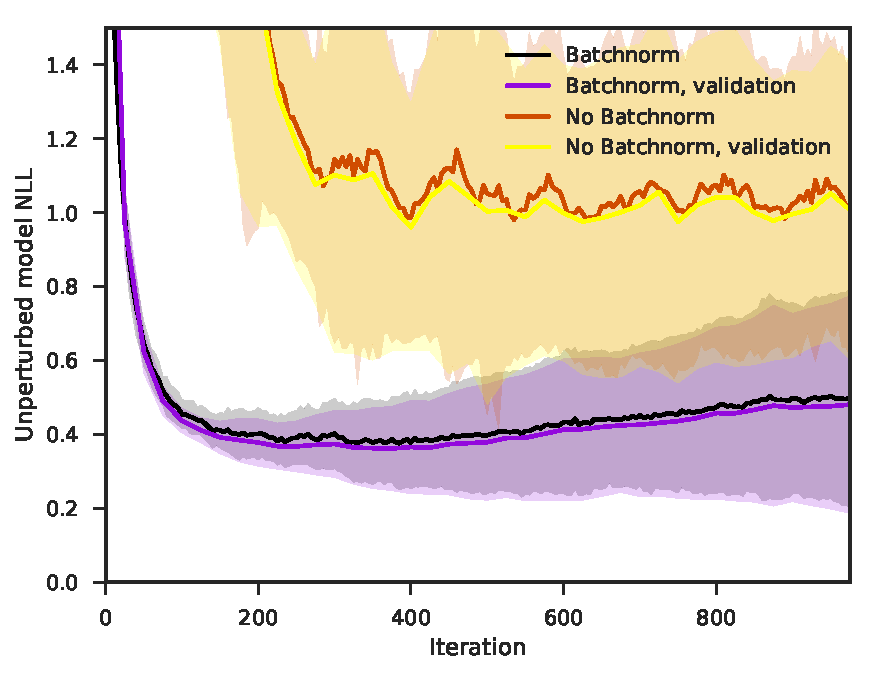
\includegraphics[height=5.8cm]{graphics/E017-bn-analysis/return_unp-all-series-mean-sd.pdf}
        \caption{}
        \label{fig: Theory: E017-bn-analysis/return_unp-all-series-mean-sd}
    \end{subfigure}
    \caption{Batch normalization experiment using the Adam optimizer.}
    \label{fig: Theory: E017-bn-analysis}
\end{figure}
\begin{figure}[tbp!]
    \begin{subfigure}[b]{0.49\textwidth}
        \centering
        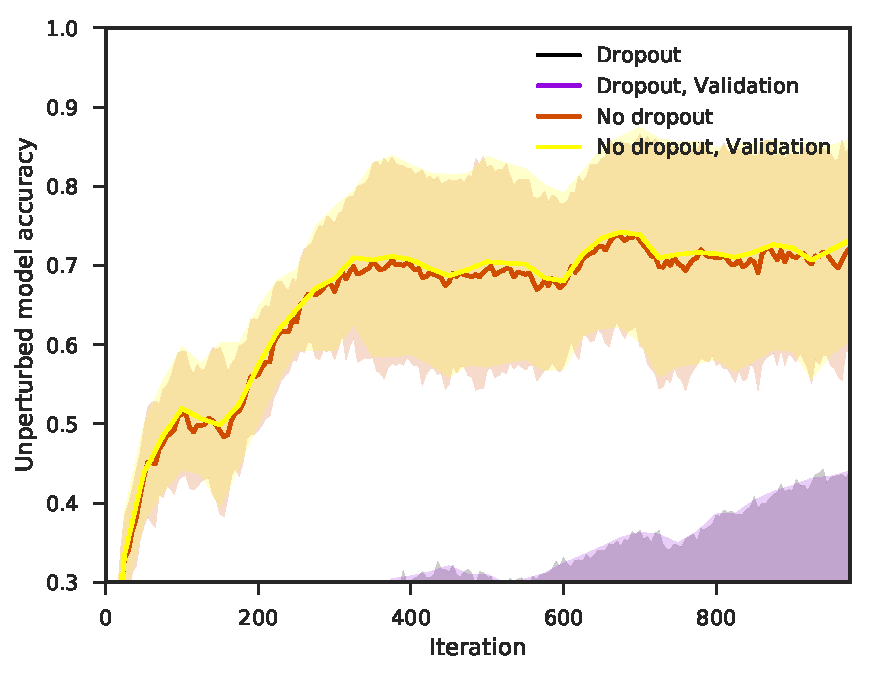
\includegraphics[height=5.8cm]{graphics/E023-DO-Adam-analysis/accuracy_unp-all-series-mean-sd.pdf}
        \caption{}
        \label{fig: Theory: E023-DO-Adam-analysis/accuracy_unp-all-series-mean-sd}
    \end{subfigure}
    \hfill
    \begin{subfigure}[b]{0.49\textwidth}
        \centering
        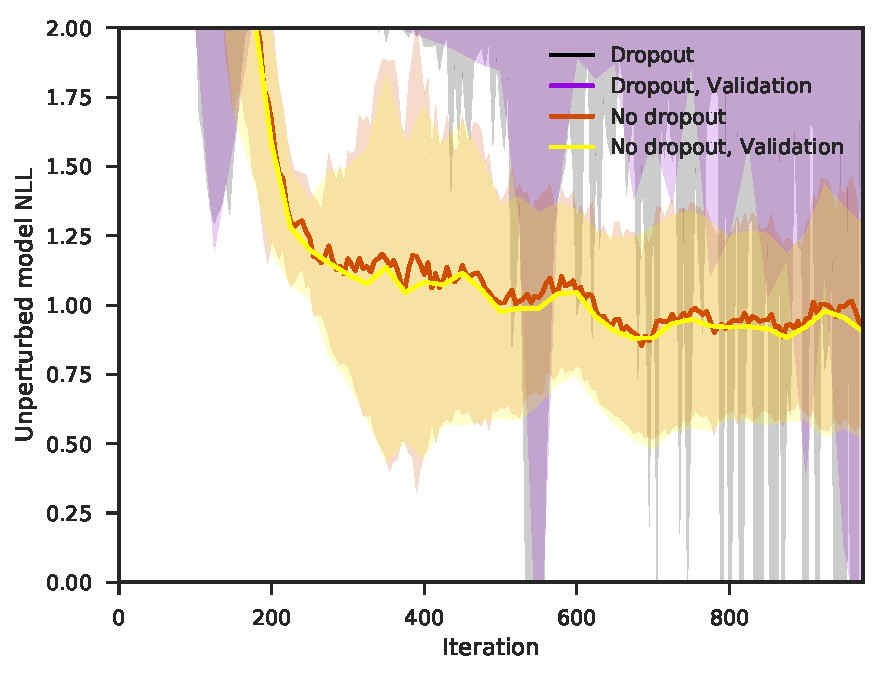
\includegraphics[height=5.8cm]{graphics/E023-DO-Adam-analysis/return_unp-all-series-mean-sd.pdf}
        \caption{}
        \label{fig: Theory: E023-DO-Adam-analysis/return_unp-all-series-mean-sd}
    \end{subfigure}
    \vspace{-0.2cm}
    \caption{Dropout experiment using the Adam optimizer.}
    \label{fig: Theory: E023-DO-Adam-analysis}
\end{figure}
\begin{figure}[tbp!]
    \begin{subfigure}[b]{0.49\textwidth}
        \centering
        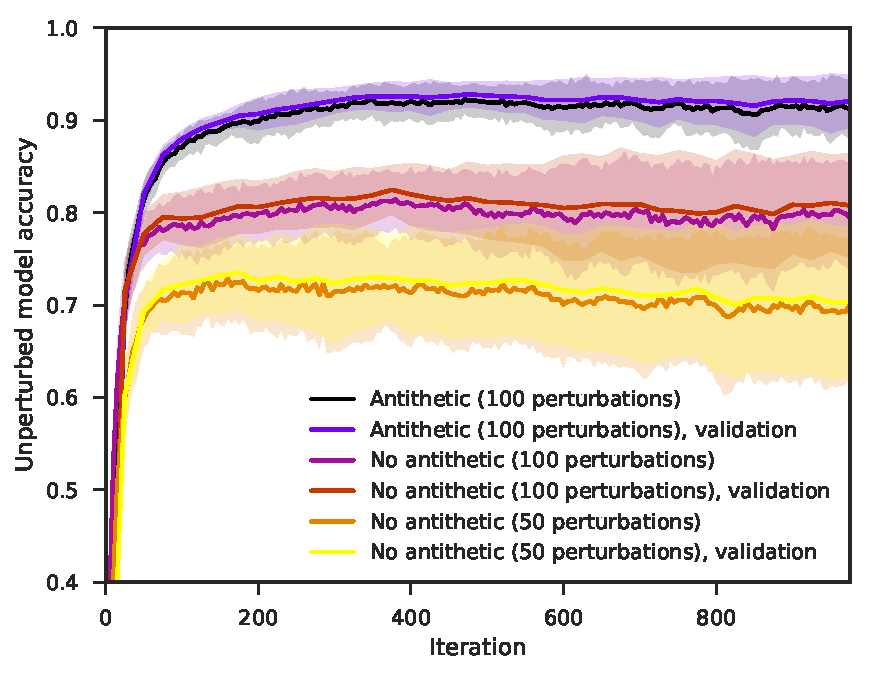
\includegraphics[height=5.8cm]{graphics/E019-AS-analysis/accuracy_unp-all-series-mean-sd.pdf}
        \caption{}
        \label{fig: Theory: E019-AS-analysis/accuracy_unp-all-series-mean-sd}
    \end{subfigure}
    \hfill
    \begin{subfigure}[b]{0.49\textwidth}
        \centering
        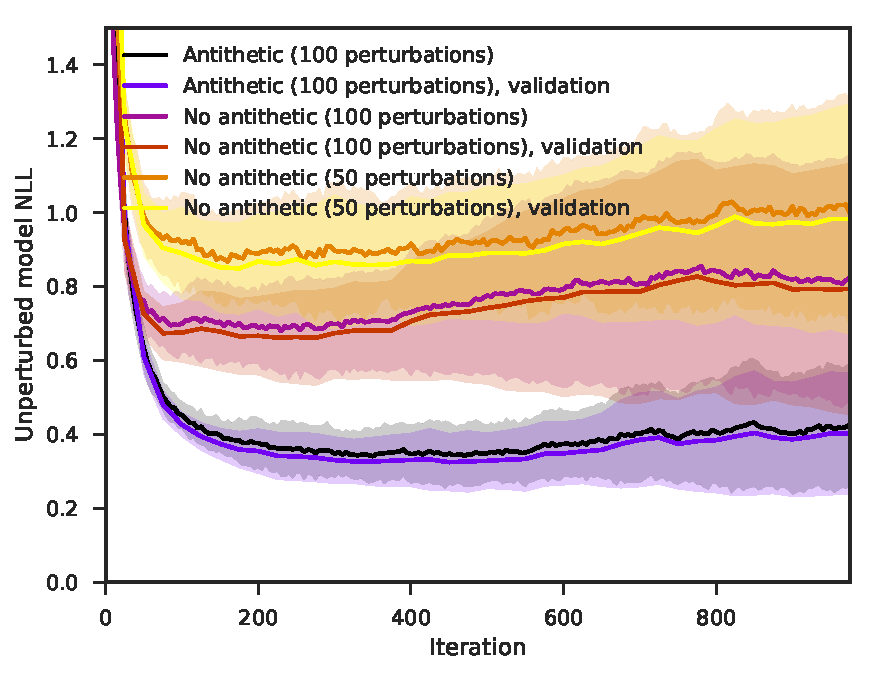
\includegraphics[height=5.8cm]{graphics/E019-AS-analysis/return_unp-all-series-mean-sd.pdf}
        \caption{}
        \label{fig: Theory: E019-AS-analysis/return_unp-all-series-mean-sd}
    \end{subfigure}
    \vspace{-0.2cm}
    \caption{Antithetic sampling experiment using the Adam optimizer.}
    \label{fig: Theory: E019-AS-analysis}
\end{figure}
\begin{figure}[tbp!]
    \begin{subfigure}[b]{0.49\textwidth}
        \centering
        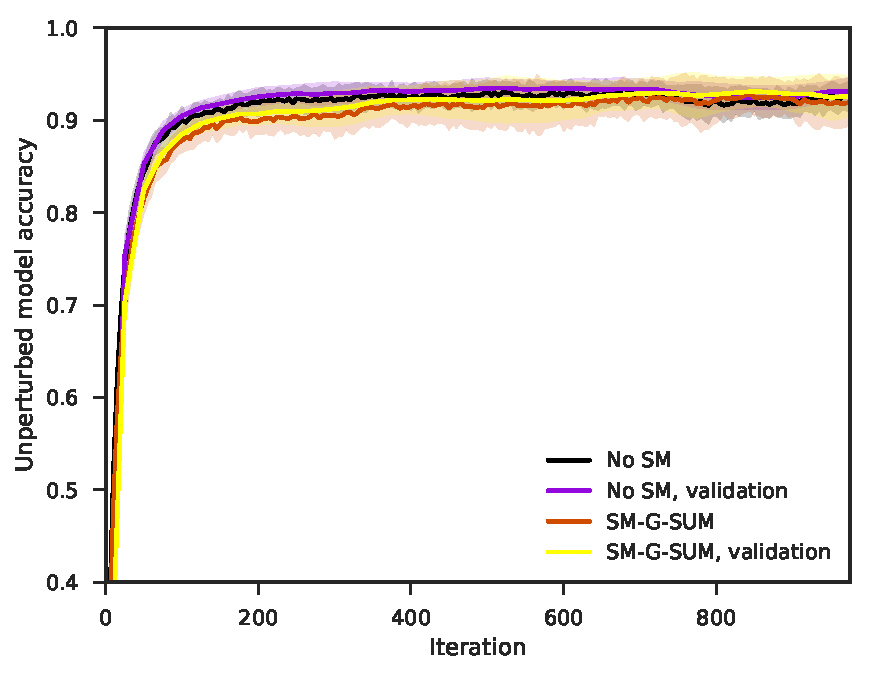
\includegraphics[height=5.8cm]{graphics/E018-SM-analysis/accuracy_unp-all-series-mean-sd.pdf}
        \caption{}
        \label{fig: Theory: E018-SM-analysis/accuracy_unp-all-series-mean-sd}
    \end{subfigure}
    \hfill
    \begin{subfigure}[b]{0.49\textwidth}
        \centering
        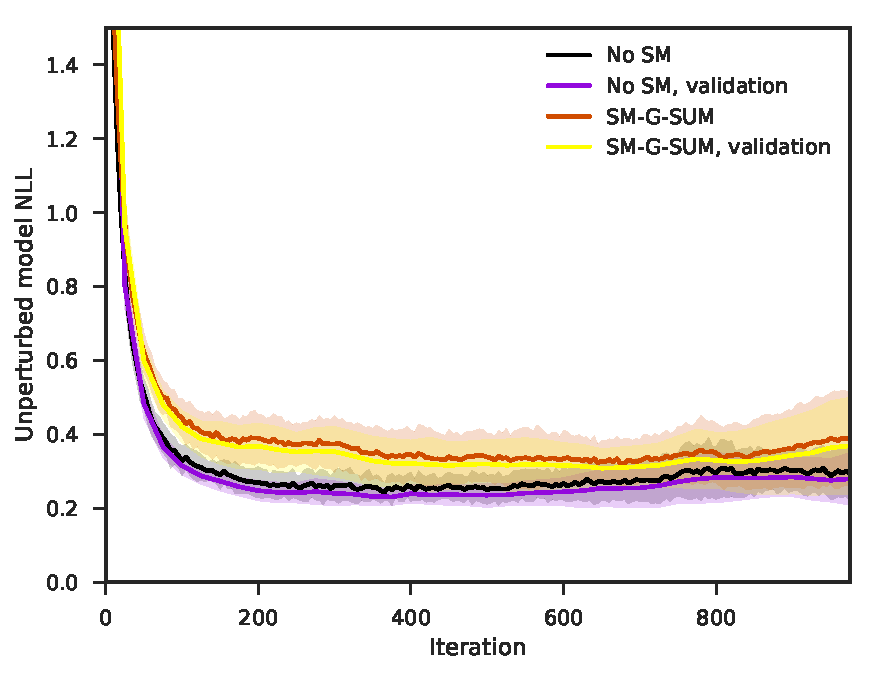
\includegraphics[height=5.8cm]{graphics/E018-SM-analysis/return_unp-all-series-mean-sd.pdf}
        \caption{}
        \label{fig: Theory: E018-SM-analysis/return_unp-all-series-mean-sd}
    \end{subfigure}
    \vspace{-0.2cm}
    \caption{Safe mutation (SM-G-SUM) experiment using the Adam optimizer.}
    \label{fig: Theory: E018-SM-analysis}
\end{figure}